\DocumentMetadata{uncompress}  % Aktivuj dekompresi PDF výstupu, která
                               % je potřeba pro správnou funkci balíčku "newpax"% Začátek preambule.
\documentclass[a4paper]{extarticle}
\usepackage{pdfpages}
\directlua{require("newpax")}  % Načti luový modul "newpax"
\usepackage{newpax}          
\newpaxsetup{usefileattributes}
\usepackage[pdfusetitle]{hyperref}

\usepackage[a4paper, margin=3cm]{geometry}
\usepackage[resetfonts]{cmap}
\usepackage{lmodern}
\usepackage[czech]{babel}
\usepackage[utf8]{inputenc}
\usepackage[T1]{fontenc}
\usepackage{url}
\usepackage[backend=biber,
            style=alphabetic,
            maxnames=5,
            alldates=iso,
            seconds=true]{biblatex} % Seznam literatury bude vygenerován 
                                    % BibLaTeXem.
\addbibresource{databaze-literatury.bib} % Seznam literatury bude vygenerován 
                             % ze zdrojů umístěných v souboru 
                             % databaze-literatury.bib.
\usepackage{imakeidx}
\makeindex

\begin{document}
\directlua{newpax.writenewpax("main")}
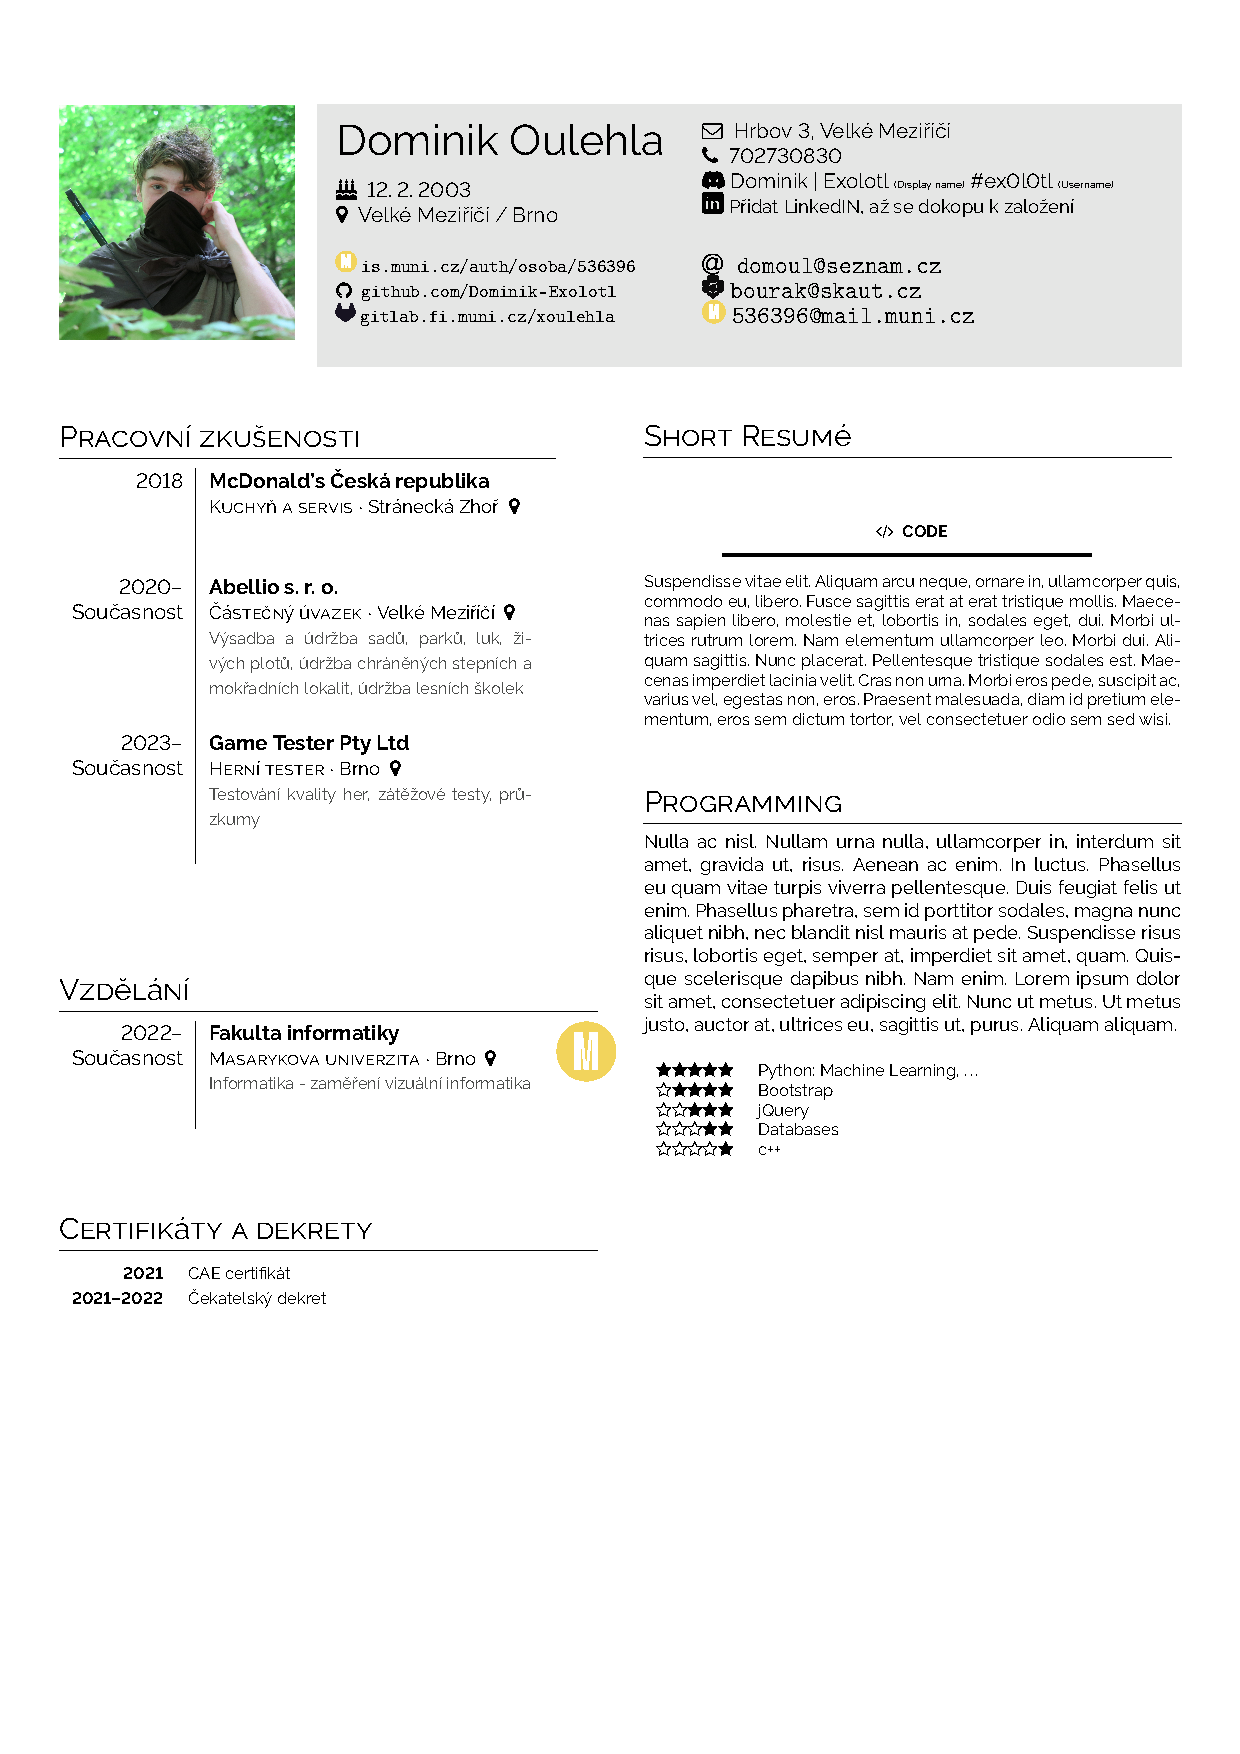
\includepdf[pages=-]{main.pdf}

\setcounter{page}{3}
\setcounter{section}{1}
\textit{Úryvek z maturitní práce:}
\section{Teoretická část}\index{Teoretická část}
\subsection{Videohry}\index{Videohry}
Videohry jsou neustále rostoucí zábavní médium, přinášející výzvy a~příběhy, nebo dokonce fungující jako umělecká díla. Jako platforma mají videohry téměř neomezené možnosti zpracovávat a~být zpracovávány tak, jak si přeje/přejí jejich autor/autoři. Proto taky bylo k~roku 2019 vydáno přes 1,1 milionu videoher \cite{games_number}, a~proto se také odhaduje, že bylo na světě k~roku 2021 3,2 miliard hráčů videoher. \cite{gamers}
\subsubsection{Herní průmysl}\index{Herní průmysl}
Herní průmysl zahrnuje vývoj a~prodej her, monetizace ve hrách, případně i~výdělek z~reklam ve videohrách.
Herní průmysl se řadí na druhé místo v~zábavním průmyslu, co se výdělku týče, s~výdělkem 160 miliard dolarů za rok 2020. \cite{media_revenue} Toto také ukazuje, že růst herního průmyslu nebyl výrazně zpomalen pandemií coronaviru, spíše naopak (ačkoliv vývoj mnoha her byl zpomalen nebo pozastaven). Růst herního průmyslu je také nejkonzistentněji a~zároveň nejrychleji rostoucí z~celého zábavního průmyslu.
Hry se podle počtu vývojářů dělí na dvě skupiny – tzv. indie a~AAA (triple-A). Zatímco triple-A hry jsou vyvíjeny vývojářskými firmami se stovkami až tisícovkami zaměstnanců, indie hry mohou být vytvořeny třeba i~jedním vývojářem (jako právě v~případě Pirates of the 31st century). Jsou to právě indie hry, které přinášejí do jistot propracovaných tripla-A her změnu, právě ony vymýšlí nové mechaniky a~posouvají hranice videoher.
\subsubsection{Historie videoher}\index{Historie videoher}
Videohry začali být vytvářeny v~40. letech 20. století. V~té době ještě nebylo možné, aby hra byla jen software přehráván na jiném zařízení, ale každá hra potřebovala svůj vlastní hardware. Tento přístup vedl ke vzniku arkádových videoher – automatů, na kterých mohli lidé hrát videohru, ke které byl automat určen. Arkádové videohry a~herny ve kterých se videohry mohli hrát dominovaly hernímu průmyslu od zveřejnění hry Pong od Atari v~1972 až do poloviny 80. let. Arkády zažily opětovný růst od 90. let po nultá léta 21. století.
Arkádové hry upadly kvůli rozšíření herních konzolí, které začali vznikat už v~70. letech, a~snižování ceny osobních počítačů, pro které byly hry vytvářené už od 50. let. Počítače a~konzole jsou stále nejvýkonnější zařízení na hraní her, proto jsou také počítačové a~konzolové hry dodnes to, co si lidé představí pod pojmem videohra.
Obrovský růst zažil videoherní průmysl v~10. letech 21. století. Díky zvětšujícímu se přístupu k~internetu a~možnosti hrát hry na něm uložené a~díky neustále se zvyšujícímu počtu lidí vlastnících chytrý telefon se vytvořili dva obrovské trhy s~videohrami – online hry a~mobilní hry, které už výdělkem překonali polovinu všech výdělků herního průmyslu. \cite{games_revenue}
\subsubsection{Žánry her, rozdělení her}\index{Žánry her, rozdělení her}
Videohry se dělí dvěma způsoby: podle platformy a~podle žánru.
Rozdělení her podle platformy je velice přímočaré – dělíme je na arkádové, počítačové, konzolové, online a~mobilní.
Podle žánru se hry dělí podle způsobu hraní na akční, střílečky, RPG, sportovní, adventury, bojové, závodní, strategické a~mnoho dalších, menších (jako třeba clicker hry). Toto rozdělení se dál větví na subžánry podle různých kritérií (například strategie na tahové a~realtime, nebo střílečky na first-person a~third-person, ale i~na taktické, battle royale a~dále). Dále se ale hry dělí i~na tématické žánry, podobně jako ostatní média, na sci-fi, fantasy, válečné, historické, hororové, či dokonce romantické.
\paragraph{Incremental (Clicker) / idle hry}\index{Incremental (Clicker) / idle hry}
Clicker je žánr hlavně počítačových, mobilních a~online her, jehož hlavním hracím prvkem je klikání, obvykle do té doby, než si klikáním hráč vydělal dost měny na nástroj, který bude klikat za něj. \cite{idle_games} Obvykle také následuje možnost vylepšovat si klikání i~již zmíněné nástroje.
První clicker hra, Progress quest, \cite{idle_games} byla vytvořena v~roce 2002, jako parodie „grindu“ (zdánlivě nekonečného získávání surovin, herní měny a~zkušeností) ve hrách žánru MMORPG (online hry na postavy pro obrovské množství hráčů). Největší popularitu ale clicker hry získali s~vydáním hry Cookie Clicker od vývojáře Orteil v~roce 2013 a~dále her jako Clicker Heroes (2014, Playsaurus), která jako nástroje pro nahrazení klikání používá různé hrdiny, kteří dále mají schopnosti, a~AdVenture Capitalist (2015, Hyper Hippo Games), která oproti Progress quest paroduje kapitalismus a~která má místo nástrojů na klikání nástroje na kupování dalších nástrojů (exponenciální růst místo lineárního)
Hry, ve kterých je klikání – a~hráčova přítomnost obecně – zapotřebí naprosto minimálně, se nazývají idle (z~anglického idle = líný). 
\paragraph{Tower defense hry}\index{Tower defense hry}
Tower defense je subžánr strategických her, v~nichž je hráčovým cílem zabránit protivnickým jednotkám, putujících po předem určené trajektorii, dosáhnout konce trasy, a~to pomocí různý obranných budov $\rightarrow$ věží (angl. tower = věž)
Ačkoliv se budoucí prvky subžánru objevovaly ve hrách už v~80. letech, první hra, která je všeobecně uznávaná jako tower defense, byla hra Rampart z~roku 1990, která ustanovila základy tower defense her – hráč na určité území pokládal obranné budovy, aby se ubránil následující fázi útoku. Tower defense hry byly také používány jako minihry ve větších hrách (Final Fantasy VI a~VII, Warcraft III). „Pytel se s~nimi roztrhl“ v~letech 2007 a~2008, kvůli tehdejšímu vzestupu internetových a~mobilních her. V~této době vyšly klasiky jako třeba Desktop Tower Defense nebo Bloons TD (Tower Defense).
Tower defense hry, ačkoliv mnohdy kombinované s~jinými žánry, vychází dodnes. Z~těch více známých: Bloons TD 6 (2018), Rock of Ages 2: Bigger \& Boulder (2017), Orcs Must Die! Unchained (2017).
\subsection{Programovací jazyky}\index{Programovací jazyky}
Programování je způsob předávání instrukcí pro splnění úkolu a~řešení problémů stroji (obvykle počítači nebo jiné výpočetní technice). Kódování je předávání těchto instrukcí přesně, pomocí binární soustavy, tedy přirozeným jazykem stroje. Konvenční programování naopak tyto instrukce předává pomocí programovacích jazyků, kterým dokáže rozumět člověk, ale i~stroj.
Programovací jazyk zajišťuje komunikaci mezi programátorem a~počítačem. Programátor skrz něj zadává příkazy, které jsou poté pomocí kompilátoru nebo interpretu předány stroji a~provedeny. 
Programovací jazyky jsou děleny podle srozumitelnosti člověkem na nižší (blízko ke strojovému kódu) a~vyšší (člověkem čitelné). 
Vyšší programovací jazyky jsou dále děleny podle programovacích paradigmat, tedy stylů, jakými kód pracuje s~prvky a~kroky programu. Takto se programovací jazyky dělí na Procedurální (naivní, strukturované a~pro hru Pirates of the 31st century nejvýznamnější – objektově orientované) a~neprocedurální (funkcionální, logické). Do tohoto výčtu by se ale také mohli zařadit programovací jazyky multiparadigmatické, tedy jazyky, které pracující s~více paradigmaty.
Programovací jazyky se dál dělí podle toho, jestli jsou příkazy vykonávané zkompilovanou verzí programu (strojovým kódem), nebo interpretovanou verzí (samo-spustitelná verze zdrojového kódu).
\subsubsection{Objektově orientované programování (OOP)}\index{Objektově orientované programování (OOP)}
Objektově orientované programování je takové programování, které při svém běhu pracuje s~tzv. objekty, kterým jsou přiřazovány funkce, které má program vykonat, a~které je možné dále propojovat nebo naopak zapouzdřit. Základem OOP tedy je, že se snaží pomocí objektů reprezentovat předměty reálného světa. OOP by se dalo označit za moderní přístup k~programování obecně.
Je mnoho programovacích jazyků, mezi jejichž paradigmata patří právě OOP: Java, C++, C\#, Visual Basic, Python, Rust
\subsubsection{Python}\index{Python}
Python je multiplatformní, multiparadigmatický programovací jazyk vyšší úrovně, poprvé vydaný v~roce 1991 programátorem Guidem van Rossumem. Je možné ho používat jak v~operačním systému Windows, tak v~Linuxu, Unixu, macOS a~dokonce Androidu. Je typický svou jednoduchostí, jednoznačností a~čitelností. Proto je nyní často používán jako první programovací jazyk mladých programátorů.
Ve svém zápise má Python méně konvencí než jiné jazyky, dokonce poskytuje dynamickou kontrolu datových typů, tedy je možné v~běhu programu v~jedné proměnné prostřídat číslo, charakter a~třeba i~dvojici seznamů. Přesto má ale Python jasně napsaná pravidla, tzv. PEP (Python Enhancement Proposal), která zajišťují čitelnost kódu, ne však jeho fungování (kód by fungoval i~bez dodržení těchto pravidel). Tato pravidla jsou například: Pro odsazování používat 4 mezery, ne tabulátor (ne velice populární pravidlo); kód má být psaný kódováním UTF-8, maximální délka řádku je 79 ad. \cite{python}

\printbibliography[heading=bibintoc]

\documentclass{modernsimplecv}
% try out different fonts: classic, fira, raleway, chivo
\usepackage[utf8]{inputenc}
\usepackage[margin=1cm, a4paper]{geometry}
\usepackage{svg}
\usepackage{xcolor}

% ------------------------------------------------------------------------------------
% you can try out different fonts here by commenting the following lines in and out
% -----------------------------------------------------------------------------------
\usepackage[default]{raleway}
%\usepackage[sfdefault]{FiraSans} %% option 'sfdefault' activates Fira Sans as the default text font\renewcommand*\oldstylenums[1]{{\firaoldstyle #1}}\normalfont
%\usepackage[familydefault,light]{Chivo} 
%\usepackage[sfdefault,light,condensed]{roboto}
%\usepackage[default]{cantarell}
%\usepackage[sfdefault]{AlegreyaSans}


\usepackage{beuron}
%\usepackage{LobsterTwo}%if not suposed to be main font, load other main font after this


%------------------------------------------------------------------ Variablen

\newlength{\rightcolwidth}
\newlength{\leftcolwidth}
\setlength{\leftcolwidth}{0.48\textwidth}
\setlength{\rightcolwidth}{0.47\textwidth}
% \colorlet{shadecolor}{gray!40}

%------------------------------------------------------------------
\title{CV-Dominik-Oulehla}
\author{Dominik Oulehla}
\date{November 2024}

\pagestyle{empty}
\begin{document}


\thispagestyle{empty}
%-------------------------------------------------------------



\tikz[remember picture,overlay] {%
\node[rectangle, fill=white, anchor=north, minimum width=\paperwidth, minimum height=5cm](header) at (current page.north){};%
}

\begin{minipage}[t]{0.21\textwidth}
\vspace{0pt} % Trick for alignment
\includegraphics[width=\textwidth]{"Profile picture - hidden.jpg"}\hspace{1em}
\end{minipage}
\hfill
\begin{minipage}[t]{0.77\textwidth}
\vspace{0pt} % Trick for alignment
\begin{shaded*}

\begin{minipage}[t]{0.4\textwidth}
\vspace{0pt} % Trick for alignment
% here the fancy font can be taken out by removing \LobsterTwo
{\par\centering\huge\textsf{Dominik Oulehla}} \\[0.3cm]
\faBirthdayCake~ 12. 2. 2003 \\
\faMapMarker~ Velké Meziříčí / Brno \\

\faEnvelopeO~ Hrbov 3, Velké Meziříčí \\

{\small
\includesvg[height=11pt]{fimu.svg} \protect\url{is.muni.cz/auth/osoba/536396} \\
\faGithub~ \protect\url{github.com/Dominik-Exolotl} \\
\includesvg[height=10pt]{gitlab-logo-600.svg} \protect\url{gitlab.fi.muni.cz/xoulehla}
}
\end{minipage}\hfill
\begin{minipage}[t]{0.55\textwidth}
\vspace{0pt} % Trick for alignment
\faPhone~ 702730830 \\ \\
\large
\faAt~ \protect\url{domoul@seznam.cz}\\
\includesvg[height=11pt]{SKAUT_logo_netext.svg} \protect\url{bourak@skaut.cz} \\
\includesvg[height=11pt]{fimu.svg} \protect\url{536396@mail.muni.cz} \normalsize\\

\end{minipage}
\hfill
\end{shaded*}
\end{minipage}\\[15pt]


%------------------------------------------------

% hier muss die "unsichtbare" Überschrift rein, weil er sonst nicht die Paracols startet... komisch...
\subsection*{}
\vspace{-3em}

\setlength{\columnsep}{1.5cm}
\columnratio{0.48}[0.47]
\begin{paracol}{2}
\hbadness5000
%\backgroundcolor{c[1]}[rgb]{1,1,0.8} % cream yellow for column-1 %\backgroundcolor{g}[rgb]{0.8,1,1} % \backgroundcolor{l}[rgb]{0,0,0.7} % dark blue for left margin

\paracolbackgroundoptions

% 0.9,0.9,0.9 -- 0.8,0.8,0.8


\footnotesize
{

\small
\section*{Short Resumé}

\begin{minipage}[t]{\leftcolwidth}
\begin{tabular}{r| p{0.6\textwidth} c}
    \cvevent{2018--2021}{Captain of the Black Pearl}{Lead}{East Indies}{Finally got the goddamn ship back. \lorem}{disney.png} \\
    \cvevent{2019}{Freelance Pirate}{Bucaneering}{Tortuga}{This and that. The usual, aye?}{medal.jpeg} \\
    \cvevent{2016--2017}{Captain of the Black Pearl}{Lead}{Tortuga}{Found a secret treasure, lost the ship.}{medal.jpeg}
\end{tabular}

\vspace{4em}

\small
\section*{Lots of Information}

\begin{tabular}{r| p{0.6\textwidth} c}
    \cvevent{2018--2021}{Captain of the Black Pearl}{Lead}{East Indies}{Finally got the goddamn ship back.}{disney.png} \\
    \cvevent{2019}{Freelance Pirate}{Bucaneering}{Tortuga}{This and that. The usual, aye? \lorem}{medal.jpeg} \\
    \cvevent{2016--2017}{Captain of the Black Pearl}{Lead}{Tortuga}{Found a secret treasure, lost the ship.}{medal.jpeg}
\end{tabular}

\vspace{4em}
\end{minipage}

\begin{minipage}[t]{\leftcolwidth}
\section*{Degrees}
\begin{tabular}{r p{0.6\textwidth} c}
    \cvdegree{1710}{Captain}{Certified}{Tortuga Uni}{}{disney.png} \\
    \cvdegree{1715}{Bucaneering}{M.A.}{London}{}{medal.jpeg} \\
    \cvdegree{1720}{Bucaneering}{B.A.}{London}{}{medal.jpeg}
\end{tabular}
\end{minipage}\hfill

\vspace{3em}

\begin{minipage}[t]{\leftcolwidth}
\section*{Certificates \& Grants}
\begin{tabular}{>{\footnotesize\bfseries}r >{\footnotesize}p{0.55\textwidth}}
    1708 & Captain's Certificates \\
    1710 & Travel grant \\
    1715--1716 & Grant from the Pirate's Company\\
    1708 & Captain's Certificates \\
    1710 & Travel grant \\
    1715--1716 & Grant from the Pirate's Company
\end{tabular}
\bigskip

\end{minipage}\hfill


\vspace{2em}

\begin{minipage}[t]{\leftcolwidth}
\section*{Lots of Information}
\begin{tabular}{r| p{0.6\textwidth} c}
    \cvevent{2018--2021}{Captain of the Black Pearl}{Lead}{East Indies}{Finally got the goddamn ship back. \lorem}{disney.png} \\
    \cvevent{2019}{Freelance Pirate}{Bucaneering}{Tortuga}{This and that. The usual, aye?}{medal.jpeg} \\
    \cvevent{2016--2017}{Captain of the Black Pearl}{Lead}{Tortuga}{Found a secret treasure, lost the ship.}{medal.jpeg}
\end{tabular}

\vspace{4em}

\small
\section*{Lots of Information}

\begin{tabular}{r| p{0.6\textwidth} c}
    \cvevent{2018--2021}{Captain of the Black Pearl}{Lead}{East Indies}{Finally got the goddamn ship back.}{disney.png} \\
    \cvevent{2019}{Freelance Pirate}{Bucaneering}{Tortuga}{This and that. The usual, aye? \lorem}{medal.jpeg} \\
    \cvevent{2016--2017}{Captain of the Black Pearl}{Lead}{Tortuga}{Found a secret treasure, lost the ship.}{medal.jpeg}
\end{tabular}

\vspace{4em}
\end{minipage}

}
%-----------------------------------------------------------
\switchcolumn

\begin{minipage}[t]{\rightcolwidth}
\section*{Short Resumé}

\begin{tabular}{r| p{0.6\textwidth} c}
    \cvevent{2018--2021}{Captain of the Black Pearl}{Lead}{East Indies}{Finally got the goddamn ship back.}{disney.png} \\
    \cvevent{2019}{Freelance Pirate}{Bucaneering}{Tortuga}{This and that. The usual, aye?}{medal.jpeg} \\
    \cvevent{2016--2017}{Captain of the Black Pearl}{Lead}{Tortuga}{Found a secret treasure, lost the ship.}{medal.jpeg}
\end{tabular}

\end{minipage}

\vspace{2em}

\lineheading{\rightcolwidth}{Code}{\faCode}{black}

\lipsum[10]



\bigskip

\section{Programming} 
{\small
\lipsum[20]

}
\bigskip

\begin{skillsection}{\rightcolwidth}
    \cvitem{\faStar\faStar\faStar\faStar\faStar}{Python: Machine Learning, \dots}
    \cvitem{\faStarO\faStar\faStar\faStar\faStar}{Bootstrap}
            \cvitem{\faStarO\faStarO\faStar\faStar\faStar}{jQuery}
        \cvitem{\faStarO\faStarO\faStarO\faStar\faStar}{Databases}
    \cvitem{\faStarO\faStarO\faStarO\faStarO\faStar}{c++}
\end{skillsection}


\bigskip



\vspace{4em}


\begin{minipage}[t]{\rightcolwidth}
\section*{Publications}
\begin{tabular}{>{\footnotesize\bfseries}r >{\footnotesize}p{0.7\textwidth}}
    1729 & \emph{How I almost got killed by Lady Swan}, Tortuga Printing Press. \\
    1720 & ``Privateering for Beginners'', in: \emph{The Pragmatic Pirate} (1/1720).\\
    1729 & \emph{How I almost got killed by Lady Swan}, Tortuga Printing Press. \\
    1720 & ``Privateering for Beginners'', in: \emph{The Pragmatic Pirate} (1/1720).\\
    1729 & \emph{How I almost got killed by Lady Swan}, Tortuga Printing Press. \\
    1720 & ``Privateering for Beginners'', in: \emph{The Pragmatic Pirate} (1/1720).
\end{tabular}
\bigskip

\section*{Talks}
\begin{tabular}{>{\footnotesize\bfseries}r >{\footnotesize}p{0.6\textwidth}}
    Nov. 1726 & ``How I lost my ship (\& and how to get it back)'', at: \emph{Annual Pirate's Conference} in Tortuga, Nov. 1726. \\
    Nov. 1726 & ``How I lost my ship (\& and how to get it back)'', at: \emph{Annual Pirate's Conference} in Tortuga, Nov. 1726. \\
    Nov. 1726 & ``How I lost my ship (\& and how to get it back)'', at: \emph{Annual Pirate's Conference} in Tortuga, Nov. 1726.
\end{tabular}
\end{minipage}









\end{paracol}

\vfill{} % Whitespace before final footer

%----------------------------------------------------------------------------------------
%	FINAL FOOTER
%----------------------------------------------------------------------------------------
\setlength{\parindent}{0pt}
\begin{minipage}[t]{\textwidth}
\begin{center}\fontfamily{\sfdefault}\selectfont \color{black!70}
{\small Jack Sparrow \icon{\faEnvelopeO}{black}{} The Black Pearl \icon{\faMapMarker}{black}{} Tortuga \icon{\faPhone}{black}{} 0099/333 5647380 
\icon{\faAt}{black}{} \protect\url{jack@sparrow.com}
}
\end{center}
\end{minipage}

\end{document}

\renewcommand{\indexname}{}
\vspace{-1.8cm}
\documentclass[a4paper]{extarticle}
\usepackage[resetfonts]{cmap}
\usepackage{lmodern}
\usepackage[czech]{babel}
\usepackage[utf8]{inputenc}
\usepackage[T1]{fontenc}
\usepackage{hyperref}
\usepackage{url}
\usepackage[backend=biber,
            style=alphabetic,
            maxnames=5,
            alldates=iso,
            seconds=true]{biblatex} % Seznam literatury bude vygenerován 
                                    % BibLaTeXem.
\addbibresource{databaze-literatury.bib} % Seznam literatury bude vygenerován 
                             % ze zdrojů umístěných v souboru 
                             % databaze-literatury.bib.

\begin{document}
\setcounter{page}{3}
\setcounter{section}{1}
\section{Teoretická část}
\subsection{Videohry}
Videohry jsou neustále rostoucí zábavní médium, přinášející výzvy a~příběhy, nebo dokonce fungující jako umělecká díla. Jako platforma mají videohry téměř neomezené možnosti zpracovávat a~být zpracovávány tak, jak si přeje/přejí jejich autor/autoři. Proto taky bylo k~roku 2019 vydáno přes 1,1 milionu videoher \cite{games_number}, a~proto se také odhaduje, že bylo na světě k~roku 2021 3,2 miliard hráčů videoher. \cite{gamers}
\subsubsection{Herní průmysl}
Herní průmysl zahrnuje vývoj a~prodej her, monetizace ve hrách, případně i~výdělek z~reklam ve videohrách.
Herní průmysl se řadí na druhé místo v~zábavním průmyslu, co se výdělku týče, s~výdělkem 160 miliard dolarů za rok 2020. \cite{media_revenue} Toto také ukazuje, že růst herního průmyslu nebyl výrazně zpomalen pandemií coronaviru, spíše naopak (ačkoliv vývoj mnoha her byl zpomalen nebo pozastaven). Růst herního průmyslu je také nejkonzistentněji a~zároveň nejrychleji rostoucí z~celého zábavního průmyslu.
Hry se podle počtu vývojářů dělí na dvě skupiny – tzv. indie a~AAA (triple-A). Zatímco triple-A hry jsou vyvíjeny vývojářskými firmami se stovkami až tisícovkami zaměstnanců, indie hry mohou být vytvořeny třeba i~jedním vývojářem (jako právě v~případě Pirates of the 31st century). Jsou to právě indie hry, které přinášejí do jistot propracovaných tripla-A her změnu, právě ony vymýšlí nové mechaniky a~posouvají hranice videoher.
\subsubsection{Historie videoher}
První videohry začali být vytvářeny v~40. letech 20. století. V~té době ještě nebylo možné, aby hra byla jen software přehráván na jiném zařízení, ale každá hra potřebovala svůj vlastní hardware. Tento přístup vedl ke vzniku arkádových videoher – automatů, na kterých mohli lidé hrát videohru, ke které byl automat určen. Arkádové videohry a~herny ve kterých se videohry mohli hrát dominovaly hernímu průmyslu od zveřejnění hry Pong od Atari v~1972 až do poloviny 80. let. Arkády zažily opětovný růst od 90. let po nultá léta 21. století.
Arkádové hry upadly kvůli rozšíření herních konzolí, které začali vznikat už v~70. letech, a~snižování ceny osobních počítačů, pro které byly hry vytvářené už od 50. let. Počítače a~konzole jsou stále nejvýkonnější zařízení na hraní her, proto jsou také počítačové a~konzolové hry dodnes to, co si lidé představí pod pojmem videohra.
Obrovské zvětšení zažil videoherní průmysl v~10. letech 21. století. Díky zvětšujícímu se přístupu k~internetu a~možnosti hrát hry na něm uložené a~díky neustále se zvyšujícímu počtu lidí vlastnících chytrý telefon se vytvořili dva obrovské trhy s~videohrami – online hry a~mobilní hry, které už výdělkem překonali polovinu všech výdělků herního průmyslu. \cite{games_revenue}
\subsubsection{Žánry her, rozdělení her}
Videohry se dělí dvěma způsoby: podle platformy a~podle žánru.
Rozdělení her podle platformy je velice přímočaré – dělíme je na arkádové, počítačové, konzolové, online a~mobilní
Podle žánru se hry dělí jednak podle způsobu hraní na akční, střílečky, RPG, sportovní, adventury, bojové, závodní, strategické a~mnoho dalších, menších (jako třeba clicker hry).Toto rozdělení se dál větví na subžánry podle různých kritérií (například strategie na tahové a~realtime, nebo střílečky na first-person a~third-person, ale i~na taktické, battle royale a~dále). Jednak se ale hry dělí i~na tématické žánry, podobně jako ostatní média, na sci-fi, fantasy, válečné, historické, hororové, či dokonce romantické.
\paragraph{Incremental (Clicker) / idle hry}
Clicker je žánr hlavně počítačových, mobilních a~online her, jehož hlavním hracím prvkem je klikání, obvykle do té doby, než si klikáním hráč vydělal dost měny na nástroj, který bude klikat za něj. \cite{idle_games} Obvykle také následuje možnost vylepšovat si klikání i~již zmíněné nástroje.
První clicker hra, Progress quest, \cite{idle_games} byla vytvořena v~roce 2002, jako parodie „grindu“ (zdánlivě nekonečného získávání surovin, herní měny a~zkušeností) ve hrách žánru MMORPG (online hry na postavy pro obrovské množství hráčů). Největší popularitu ale clicker hry získali s~vydáním hry Cookie Clicker od vývojáře Orteil v~roce 2013 a~dále her jako Clicker Heroes (2014, Playsaurus), která jako nástroje pro nahrazení klikání používá různé hrdiny, kteří dále mají schopnosti, a~AdVenture Capitalist (2015, Hyper Hippo Games), která oproti Progress quest paroduje kapitalismus a~která má místo nástrojů na klikání nástroje na kupování dalších nástrojů (exponenciální růst místo lineárního)
Hry, ve kterých je klikání – a~hráčova přítomnost obecně – zapotřebí naprosto minimálně, se nazývají idle (z~anglického idle = líný). 
\paragraph{Tower defense hry}
Tower defense je subžánr strategických her, v~nichž je hráčovým cílem zabránit protivnickým jednotkám, putujících po předem určené trajektorii, dosáhnout konce trasy, a~to pomocí různý obranných budov -> věží (angl. tower = věž)
Ačkoliv se budoucí prvky subžánru objevovaly ve hrách už v~80. letech, první hra, která je všeobecně uznávaná jako tower defense, byla hra Rampart z~roku 1990, která ustanovila základy tower defense her – hráč na určité území pokládal obranné budovy, aby se ubránil následující fázi útoku. Tower defense hry byly také používány jako minihry ve větších hrách (Final Fantasy VI a~VII, Warcraft III). „Pytel se s~nimi roztrhl“ v~letech 2007 a~2008, kvůli tehdejšímu vzestupu internetových a~mobilních her. V~této době vyšly klasiky jako třeba Desktop Tower Defense nebo Bloons TD (Tower Defense).
Tower defense hry, ačkoliv mnohdy kombinované s~jinými žánry, vychází dodnes. Z~těch více známých: Bloons TD 6 (2018), Rock of Ages 2: Bigger \& Boulder (2017), Orcs Must Die! Unchained (2017).
\subsection{Programovací jazyky}
Programování je způsob předávání instrukcí pro splnění úkolu a~řešení problémů stroji (obvykle počítači nebo jiné výpočetní technice). Kódování je předávání těchto instrukcí přesně, pomocí binární soustavy, tedy přirozeným jazykem stroje. Konvenční programování naopak tyto instrukce předává pomocí programovacích jazyků, kterým dokáže rozumět člověk, ale i~stroj (za pomoci kompilátoru daného jazyku, který ho převede do binární soustavy).
Programovací jazyk zajišťuje komunikaci mezi programátorem a~počítačem. Programátor skrz něj zadává příkazy, které jsou poté pomocí kompilátoru nebo interpretu předány stroji a~provedeny. 
Programovací jazyky jsou děleny podle srozumitelnosti člověkem na nižší (blízko ke strojovému kódu) a~vyšší (člověkem čitelné). 
Vyšší programovací jazyky jsou dále děleny podle programovacích paradigmat, tedy stylů, jakými kód pracuje s~prvky a~kroky programu. Takto se programovací jazyky dělí na Procedurální (naivní, strukturované a~pro hru Pirates of the 31st century nejvýznamnější – objektově orientované) a~neprocedurální (funkcionální, logické). Do tohoto výčtu by se ale také mohli zařadit programovací jazyky multiparadigmatické, tedy jazyky, které pracující s~více paradigmaty.
Programovací jazyky se dál dělí podle toho, jestli jsou příkazy vykonávané zkompilovanou verzí programu (strojovým kódem), nebo interpretovanou verzí (samo-spustitelná verze zdrojového kódu).
\subsubsection{Objektově orientované programování (OOP)}
Objektově orientované programování je takové programování, které při svém běhu pracuje s~tzv. objekty, kterým jsou přiřazovány funkce, které má program vykonat, a~které je možné dále propojovat nebo naopak zapouzdřit. Základem OOP tedy je, že se snaží pomocí objektů reprezentovat předměty reálného světa. OOP by se dalo označit za moderní přístup k~programování obecně.
Je mnoho programovacích jazyků, mezi jejichž paradigmata patří právě OOP: Java, C++, C\#, Visual Basic, Python, Rust
\subsubsection{Python}
Python je multiplatformní, multiparadigmatický programovací jazyk vyšší úrovně, poprvé vydaný v~roce 1991 programátorem Guidem van Rossumem. Je možné ho používat jak v~operačním systému Windows, tak v~Linuxu, Unixu, macOS a~dokonce Androidu. Je typický svou jednoduchostí, jednoznačností a~čitelností. Proto je nyní často používán jako první programovací jazyk mladých programátorů.
Ve svém zápise má Python méně konvencí než jiné jazyky, dokonce poskytuje dynamickou kontrolu datových typů, tedy je možné v~běhu programu v~jedné proměnné prostřídat číslo, charakter a~třeba i~dvojici seznamů. Přesto má ale Python jasně napsaná pravidla, tzv. PEP (Python Enhancement Proposal), která zajišťují čitelnost kódu, ne však jeho fungování (kód by fungoval i~bez dodržení těchto pravidel). Tato pravidla jsou například: Pro odsazování používat 4 mezery, ne tabulátor (ne velice populární pravidlo); kód má být psaný kódováním UTF-8, maximální délka řádku je 79 ad. \cite{python}

\printbibliography[heading=bibintoc]

\end{document}


\end{document}

\end{document}